\section{Conclusão}\label{sec:conclusion}
A aplicação desenvolvida já permite a interação com a extensão, que atualmente está disponível como pacote local. Ela conta com controle de acesso via \textit{Magic Login} e acesso condicional baseado no perfil do usuário, garantindo que o aluno atue apenas como monitorado, enquanto o docente mantém o papel de criador de aula.

Além disso, a extensão já realiza a captura dos logs de atividade, conforme ilustrado na Figura~\ref{fig:figura4}. Com isso, a etapa de mineração dos dados, que servem de base para os relatórios, foi concluída com êxito. Esses resultados representam uma etapa inicial do projeto, mas já permitem avaliar a viabilidade técnica da solução.

\FloatBarrier
\begin{figure}[H]
\centering
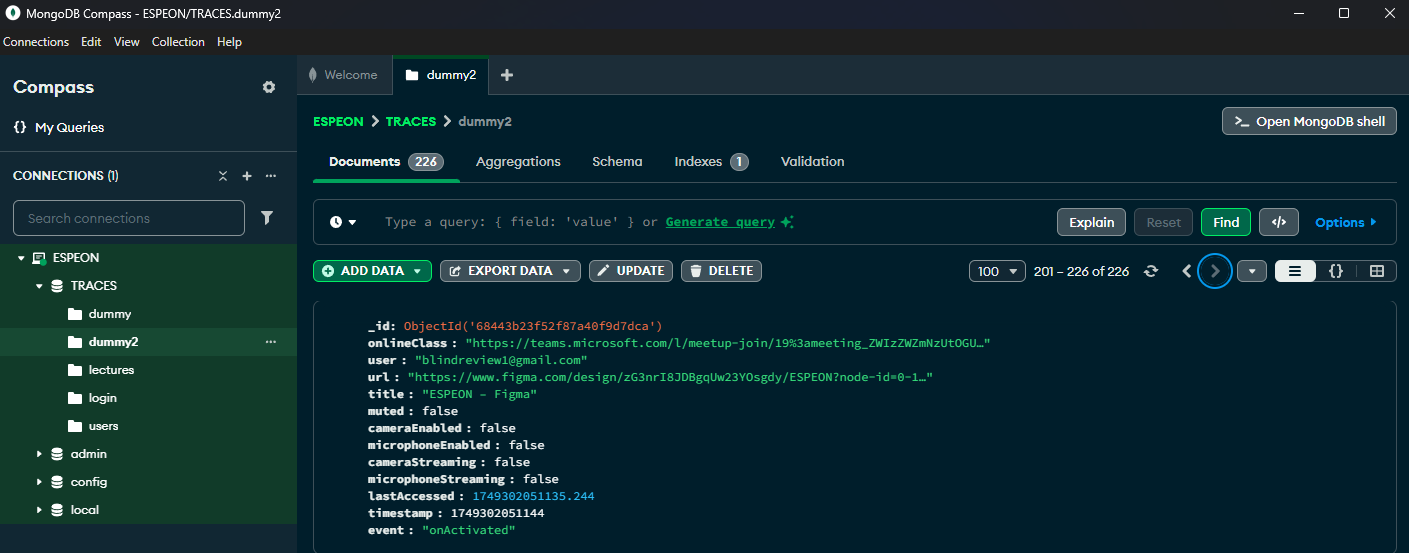
\includegraphics[width=.99\textwidth]{assets/images/resultadosv2.png}
\caption{Exemplo de \textit{Payload} Coletado}
\label{fig:figura4}
\end{figure}


\subsection{Trabalhos Futuros}\label{sub:future_endeavors}
As próximas etapas do projeto envolvem avanços em infraestrutura, coleta e análise de dados. Inicialmente, será realizada a implantação da API Flask em ambiente de produção, juntamente com a migração do banco de dados MongoDB para uma instância AtlasDB. Em seguida, a extensão será publicada na Chrome Web Store.

Após a implantação, será implementada a rotina de geração de relatórios, a partir da análise dos \textit{logs} emitidos pela extensão. Esses relatórios serão convertidos em documentos gráficos e exportados em formato PDF.

Na fase final, será feita a coleta de dados por meio de testes laboratoriais com docentes e discentes. A análise da efetividade das aulas será baseada nas métricas obtidas, permitindo a identificação de possíveis tendências comportamentais entre os participantes.

